
\chapter{Podstawy teoretyczne}

W rozdziale tym przedstawiony zostanie przegląd literatury, który stanowi podstawy wiedzy na temat eksploracji danych, a w szczególności problemu odkrywania reguł asocjacyjnych w dużych zbiorach danych. Zebrana wiedza posłużyła autorowi do opracowania algorytmu wykorzystującego możliwości współczesnych kart graficznych.

\section{Definicje}

\subsection{Model teoretyczny}

Niech $I = \lbrace i_1,i_2,...,i_m \rbrace$ będzie \emph{zbiorem elementów} o liczności $|I| = m$. \emph{Transakcją} nazwano dowolny, niepusty podzbiór $X \subseteq I$ zbioru elementów. Bazą danych $DB$ nazwano dowolny zbiór par $(id, X)$, gdzie $X$ jest transakcją, a $id$ jest dowolną wartością unikalną w ramach bazy danych nazywaną \emph{identyfikatorem transakcji}. Bez utraty ogólności założono iż $id\in \mathbb{N}$. 

\emph{Wsparciem} (\english{support}) $sup(X)$ transakcji $X$, w bazie danych nazwano częstość wystąpień transakcji w bazie danych. Formalnie przedstawia to wzór~\ref{support:def}.

\begin{equation}
\label{support:def}
sup(X)=\frac{| \lbrace id: (id,Y)\in DB \wedge X\subseteq Y \rbrace |}{|DB|}
\end{equation} 

Łatwo zauważyć, że jeśli poziom ten jest niski, to oznacza to, że nie ma jednoznacznych dowodów na łączne występowanie elementów zbioru $Z = X \cup Y$, ponieważ zbiór $Z$ występuje w niewielkiej liczbie transakcji. 

\begin{df}\label{regula:def}
Niech będą dane dwie transakcje $X$ i $Y$ takie, że $X\cap Y=\emptyset$. Implikację postaci $X\Rightarrow  Y$ nazwano \emph{regułą asocjacyjną}.
\end{df}

\emph{Poziom ufności} (\english{confidence}) jest miarą zdefiniowaną dla implikacji reprezentowanej przez regułę asocjacyjną~\cite{Elmasri:db}. 

\begin{df}\label{confidence:def}
Pioziom ufności ($conf$) reguły asocjacyjnej $X \Rightarrow Y$ jest równy 
\begin{equation}
	conf(X \Rightarrow Y) = \frac{sup(X \cup Y)}{sup(X)}
\end{equation}
\end{df}

Po analizie definicji~\ref{confidence:def} łatwo zauważyć, że poziom ufności może być interpretowany, jako estymacja prawdopodobieństwa $P(Y | X)$.


Reguły asocjacyjne zazwyczaj powinny spełniać pewne wymagania zdefiniowane przez użytkownika - minimalne wsparcie oraz minimalny poziom ufności, oznaczane odpowiednio $minsup$ oraz $minconf$. Wyznaczają one dla aplikacji progi, jakie powinny spełniać zbiory oraz reguły, aby były brane pod uwagę w trakcie analizy.

\begin{df}
Zbiorem częstym $X \subseteq I$ nazywamy taki zbiór, który spełnia zależność $sup(X) \geq minsup$.
\end{df}

Generowanie reguł asocjacyjnych zazwyczaj sprowadza się do dwóch, niezależnych kroków:
\begin{enumerate}
	\item Minimalne wsparcie jest używane do odnalezienia wszystkich zbiorów częstych w bazie danych $DB$.
	\item Znalezione zbiory często oraz minimalny poziom ufności są używane do wygenerownia reguł asocjacyjnych.
\end{enumerate}

Znalezienie wszystkich zbiorów częstych w bazie danych $DB$ jest zadaniem wymagającym przeszukania wszystkich możliwych kombinacji bez powtórzeń ze zbioru $I$. Zbiór możliwych zbiorów elementów ma liczność równą $2^n - 1$ (wszystkie zbiory, poza zbiorem pustym, który nie jest w tym wypadku zbiorem sensownym w znaczeniu poddania go analizie). 

Warto zauważyć, że dla każdego zbioru częstego $Y$, każdy jego podzbiór $X$ jest również zbiorem częstym~\cite{Problem:Statement}. Korzystając z tej właściwości wsparcia możliwe jest w sposób efektywny znalezienie wszystkich zbiorów częstych w zadanej bazie danych - z tej zależności korzysta algorytm apriori opisany w rozdziale~\ref{apriori:section}. Dodatkowo, wszystkie reguły zbudowane na podstawie zbioru częstego $Y$ muszą spełniać warunek minimalnego wsparcia, ponieważ spełnia ten warunek zbiór $Y$, a suma zbiorów reguły jest zbiorem wyjściowym $Y$.

\section{Aktualna wiedza}
W rozdziale tym zebrana została oraz opracowana dotychczasowa wiedza (\english{state-of-the-art}) na temat odkrywania reguł asocjacyjnych. Przedstawione zostaną dwa podstawowe algorytmy wykorzystywane w tym procesie: Apriori oraz FP-growth. W chwili obecnej te dwa algorytmy stanowią podstawę, na której budowane są nowe algorytmy, wykorzystujące możliwości współczesnych algorytmów (\emph{Czy wymieniać tutaj przykłady algorytmów, które bazują na nich + refy do kilku artykułów?}).

\subsection{Algorytm Apriori}\label{apriori:section}
Pierwszy algorytm odkrywający reguły asocjacyjne został przedstawiony w roku 1994 w pracy~\cite{Apriori:Main}. Niżej przedstawione zostaną szczegóły działania tego algorytmu nazwanego algorytmem \emph{Apriori}.

Zagadnienie odkrywania reguł asocjacyjnych można podzielić na dwa etapy~\cite{Problem:Statement}:
\begin{enumerate}
	\item Odkrywanie zbiorów częstych, których wartość wsparcia jest wyższa od wartości $minsup$.
	\item Generowanie reguł asocjacyjnych na podstawie znalezionych zbiorów częstych. Reguła $X \Rightarrow Y$ jest wynikiem działania algorytmu dla zbioru $Z = X \cup Y$, jeżeli spełnia ona nierówność $conf(X \Rightarrow Y) \geq minconf$. Ponieważ zbiór $Z = X \cup Y$ jest zbiorem częstym, to reguła spełnia również warunek przekraczania minimalnego wsparcia.

	Na tym etapie możliwe jest tworzenie reguł, w których w zbiorze \emph{poprzedników} ($X$ z oznaczeń z definicji~\ref{regula:def}) jest wiele elementów oraz jeden w \emph{następniku} (zbiór $Y$ z definicji~\ref{regula:def})~\cite{Problem:Statement} lub dopuszczana jest możliwość wielu elementów również w następniku~\cite{Apriori:Main}. W niniejszej pracy analizowany jest sposób generowania reguł, w którym oba zbiory mogą być zbiorami wieloelementowymi.
\end{enumerate}

W kolejnych podrozdziałach przedstawione zostaną etapy tworzące razem algorytmy Apriori.

\subsubsection{Generowanie zbiorów częstych}\label{apriori:gen}
W celu wyznaczenia zbiorów częstych algorytm dokonuje analizy bazy danych $DB$, by w kolejnych iteracjach generować rodziny coraz to liczniejszych zbiorów, będących zbiorami częstymi dla zadanej wartości $minsup$. Algorytm zaczyna od znalezienia wszystkich zbiorów jednoelementowych, które są zbiorami częstymi. W każdym kolejnym kroku generowane są zbiory częste na podstawie zbiorów wygenerowanych w kroku poprzednim. Proces ten jest kontynuowany do momentu aż nie zostaną znalezione żadne zbiory częste.

Algorytm generuje zbiory kandydatów jedynie na podstawie zbiorów częstych odkrytych w kroku poprzednim - co ważne generowanie ich odbywa się bez wielokrotnego przeglądania bazy danych transakcji. Intuicja podpowiada, że każdy podzbiór zbioru częstego jest zbiorem częstym. Zatem, każdy zbiór częsty zawierający $k$ elementów może być wygenerowany na podstawie połączenia dwóch zbiorów posiadających $k-1$ elementów, a na koniec kasując te zbiory, których jakikolwiek podzbiór nie jest częsty~\cite{Apriori:Main}.

\begin{table}
	\centering
	\begin{tabular}{|c|p{7.7cm}|} \hline
	$k$-zbiór & Zbiór zawierający $k$ elementów. \\ \hline
	$L_k$ & Zbiór zawierający $k$-zbiory. Każdy zbiór zawarty w $L_k$ zawiera dwa pola: i) zbiór oraz ii) wartość $support$. \\ \hline
	$C_k$ & Zbiór $k$-zbiorów kandydatów (potencjalnych zbiorów częstych). Każdy zbiór zawarty w $C_k$ zawiera dwa pola: i) zbiór oraz ii) wartość $support$. \\ \hline
	\end{tabular}\label{skroty:znaczanie}
	\caption{Oznaczenie skrótów w opisie algorytmu}
\end{table}

Tabela~\ref{skroty:znaczanie} zawiera spis oznaczeń używanych w opisie algorytmu. 

Procedura \proc{Apriori Frequent Set Generaion} przedstawia pseudokod realizujący opisywany w tym rozdziale algorytm generowania zbiorów częstych.

\begin{codebox}
	\Procname{$\proc{Apriori Frequent Set Generaion}$}\label{apriori:listing}
	\li $\id{L_1} \gets \lbrace 1$-zbiory częste $\rbrace$
		\li \For $(k = 2; \id{L_{k-1}} \neq \emptyset; k++)$
		\li \Do
			 $\id{C_k} \gets aprioriGen(\id{L_{k-1}})$
			\li \For \textbf{each} trasakcja $t \in \id{DB}$
			\li \Do
					$C_t \gets subset(C_k, t)$
					\li \For \textbf{each} kandydat $c \in \id{C_t}$
					\li \Do c.count++
					\End
				\End
			\li $L_k \gets \lbrace c \in C_k | c.count \geq minsup \rbrace$	
		\End
	\li Answer $\gets \bigcup_k L_k $
\end{codebox}

\paragraph{Procedura aprioriGen}
Procedura \id{aprioriGen} reprezentuje proces twórzenia zbiorów $k$-elementowych kandydatów na podstawie zbiorów wejściowych ${k-1}$-elementowych. Procedura ta jest podzielona na dwa etapy: łączenia oraz przycinania. 

Jak łatwo zauważyć wynikiem działania \proc{Join Step} są zbiory $k$-elementowe, które powstały na podstawie zbiorów wejściowych $L_{k-1}$, a ich zawartość różni się tylko jednym elementem - ostatnim. Ważnym faktem jest to, iż elementy w zbiorach są uporządkowane leksykograficzne, co wykorzystywane jest w tej procedurze.

\begin{codebox}
	\Procname{$\proc{Join Step}$}
	\li \textbf{insert into} $C_k$
	\li \textbf{select} p.item$_1$, p.item$_2$, \dots, p.item$_{k-1}$, q.item$_{k-1}$
	\li \textbf{from} $L_{k-1}$ p, $L_{k-1}$ q
	\li \textbf{where} p.item$_1 = $ q.item$_1$, \dots, p.item$_{k-2}$ = q.item$_{k-2}$, p.item$_{k-1}$ $<$ q.item$_{k-1}$
\end{codebox}

Warto zauważyć, że \proc{Join Step} jest ekwiwalentem rozszerania zbioru $L_{k-1}$ każdym elementem zbioru elementów $I$, a następnie kasowania tych $(k-1)$-zbiorów otrzymanych przez usuwanie $(k-1)$ elementu, które nie są w $L_{k-1}$. 

Warunek p.item$_{k-1}$ $<$ q.item$_{k-1}$ zapewnia, że nie będą generowane duplikaty. Dlatego też po etapie łączenia zachodzi zależność $C_k \supseteq L_k$.

Następnym krokiem jest \proc{Prune Step}, w którym usuwane są wszystkie elementy $c \in C_k$, którego jakikolwiek podzbiór $(k-1)$-elementowy zbioru $c$ nie należy do $L_{k-1}$.

\begin{codebox}
	\Procname{$\proc{Prune Step}$}
		\li \For \textbf{each} zbiór $c \in C_k$ 
		\li \Do
			\li \For \textbf{each} $(k-1)$-podzbiór s zbioru $c$
					\li \Do 
						\If $s \notin L_{k-1}$
						\li \Then
							\textbf{delete} $c$ z $C_k$
						\End
					\End
		\End
\end{codebox}

Celem operacji przycinania (\english{prune}) jest ograniczenie rozmiaru zbioru $C_k$ przed sprawdzeniem wsparcia dla kandydatów w bazie danych $DB$. W tym celu wykorzystywana jest właściwość, z której wynika, że jeśli jakiś $(k-1)$-podzbiór danego kandydata ($c \in C_k$) nie występuje w $L_{k-1}$, to kandydatk $c$ nie jest zbiorem częstym i powinien być usunięty z $C_k$.

\subsubsection{Generowanie reguł asocjacyjnych}
Po zakończeniu pierwszego etapu algorytm przystępuje do drugiego, czyli do budowania reguł asocjacyjnych na podstawie odkrytych zbiorów. Podobnie, jak w~\cite{Apriori:Main} algorytm będący przedmiotem analizy niniejszej pracy, generuje wszystkie możliwe reguły asocjacyjne dla zadanego zbioru. Mniej ogólny sposób generowania reguł został przedstawiony w pracy~\cite{Problem:Statement}, jednakże podjęto decyzję, że jest to sposób zbyt mało użyteczny w środowisku produkcyjnym.

Aby wygenerować reguły, dla każdego zbioru częstego $l$ znajdowane są niepuste podzbiory - podzbiór taki oznaczony jest jako $a$. Dla takich oznaczeń wygenerowna zostanie reguła $a \Rightarrow (l-a)$, jeżeli spełniona jest nierówność $\frac{support(l)}{support(a)} \geq minconf$. Warto zauważyć, że dla każdego zbioru częstego generowane są wszystkie możliwe niepuste podzbiory - zapewnia to, że odkryte zostaną wszystkie możliwe reguły.

Procedura~\proc{Generate Frequent Itemsets} prezentuje generowanie reguł asocjacyjnych na podstawie odkrytych zbiorów częstych.

\begin{codebox}
	\Procname{$\proc{Generate Frequent Itemsets}$}
		\li \For \textbf{each} zbiór częsty $l_k$, $k \geq 2$ 
		\li \Do
			\textbf{call} genrules($l_k$, $l_k$)
			\End
		\End
\end{codebox}

W powyższym algorytmie wykorzystana została funkcja \proc{Genrules}, która na podstawie dwóch zbiorów generuje reguły asocjacyjne. Zapis pseudokodu tej funkcji przedstawiony jest poniżej.

\begin{codebox}
	\Procname{$\proc{Genrules}$($l_k$: $k$-zbiór częsty, $a_m$: $m$-zbiór częsty)}
		\li $\id{A} \gets \lbrace (m-1)$-zbiór $a_{m-1} | a_{m-1} \subset a_m \rbrace$
		\li \For $a_{m-1} \in A$
			\li \Do
			$\id{conf} \gets \frac{support(l_k)}{support(a_{m-1})}$
			\li \If $\id{conf} \geq \id{minconf}$
				\li \Then
						\textbf{output} reguła $a_{m-1} \Rightarrow (l_k - a_{m-1})$ \\ ufność = $conf$ oraz wsparcie= $support(l_k)$
						\li \If $m-1 > 1$ 
							\li \Then
							\textbf{call} genrules($l_k$, $a_{m-1}$) \\ generowanie reguł podzbiorów zbioru $a_{m-1}$
						\End
				\End
			\End
		\End
\end{codebox}

\subsection{Algorytm FP-growth}

Podstawową wadą algorytmu Apriori jest wysoki koszt przetważania dużych zbiorów danych. Przykładowo, dla $10^4$ 1-zbiorów częstych, algorytm Apriori wygeneruje około $10^7$ 2-zbiorów kandydatów, które następnie poddane zostaną weryfikacji, czy są zbiorami częstymi. Poza tym algorytm ten wymaga wielokrotnego odczytywania zawartości bazy danych - w każdym kroku algorytmu należy odczytać całą bazę danych w celu obliczenia wsparcia zbiorów kandydujących.

Wymienione wyżej wady algorytmu Apriori nie występują w algorytmie \emph{FP-growth} przedstawionym w pełni w pracy~\cite{Main:FPgrowth}. Algorytm ten pozwala wyeliminować konieczność generowania tak dużej liczby kandydujących zbiorów elementów oraz ogranicza liczbę dostępu do bazy danych do absolutnego minimum.  Co więcej algorytm ten harakteryzuje się kompletnością, co oznacza, że znajdowane są wszystkie wzorce o określonej częstości.

Algorytm FP-growth można podzielić na trzy podstawowe kroki.
\begin{enumerate}
	\item W kroku pierwszym generowana jest skompresowana wersja bazy danych $DB$, mająca postać drzewa częstych wzorców.
	\item Drugim krokiem jest transformacja tak skonstruowanego drzewa do postaci \emph{FP-drzewa} (patrz definicja~\ref{fptree:def}).
	\item Trzeci krok polega na analizie FP-drzewa celem odnalezienia reguł asocjacyjnych. W kroku tym stosowana jest metoda dziel i zwyciężaj (\english{divide-and-conquer}) zamiast podejścia Apriori, czyli generowania na każdym poziomie zbioru kandydatów na zbiory częste, a następnie odcinaniu kandydatów nie spełniających kryteriów akceptacji. Takie podejście przekształca problem znajdowania długich reguł w problem szukania krótszych, a następnie konkatenacji wyników. 
\end{enumerate}

\begin{df}\label{fptree:def}
FP-drzewo (\english{frequent-pattern tree}) jest to ukorzeniony, etykietowany w wierzchołkach graf acykliczny spełniający poniższe cechy.
\end{df}
\begin{enumerate}
	\item Korzeniem drzewa jest jeden element \id{null}, zbiór poddrzew prefiksowanych elementami (jako dzieci elementu \id{null}) oraz tablicy nagłówkowej zawierającej wpisy \id{element} $\rightarrow$ \emph{wskaźnik na element drzewa}.
	\item Każdy wierzchołek poddrzewa składa się z trzech elementów: nazwy elementu (\english{item name}), licznika (\english{count}) oraz wskaźnika na inny wierzchołek. Nazwa elementu (\id{itemName}) w sposób jednoznaczny identyfikuje element ze zbioru elementów $I$, licznik przechowuje liczbę transakcji reprezentowanych przez ścieżkę od \id{null} do tego elementu, natomiast wskaźnik wskazuje na kolejny wierzchołek w FP-drzewie, którego nazwa jest identyczna do danego.
	\item Każdy wpis w tablicy nagłówkowej (\english{frequent-item-header table}) skałada się z dwóch elementów: nazwy elementu oraz wskaźnika na pierwszy element w drzewie posiadający identyczną nazwę.
\end{enumerate}

Rysunek~\ref{rys:fptree} przedstawia przykładowe FP-drzewo wraz z tablicą nagłówkową.

\begin{figure}[h]
\centering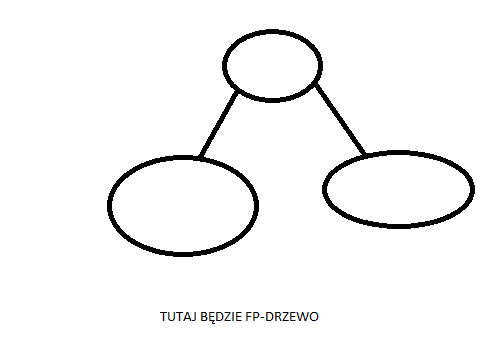
\includegraphics{figures/fptree.png}
\caption{Ilustracja przykładowego FP-drzewa}\label{rys:fptree}
\end{figure}

\subsubsection{Kompresja bazy danych}
Pierwszy etap polega na znalezieniu wszystkich $1$-zbiorów częstych występujących w bazie danych $DB$. Po ich odnalezieniu ($F_1$ - zbiór znalezionych $1$-zbiorów częstych) z każdej transakcji $T$ usuwany jest ten element, który nie należy do $F_1$. 

W wyniku usunięcia elementów nie tworzących jednoelementowych zbiorów częstych, baza ma zazwyczaj znacznie mniejszy rozmiar niż wyjściowa baza danych. Dodatkowo w tym kroku elementy w każdej transakcji zostają posortowane według maljącej wartości ich wsparcia.


\subsubsection{Konstrukcja FP-drzewa}\label{fptree:construction}
\begin{alg}\label{alg:fptre:econstruction}
	\emph{Konstrukcja FP-drzewa}.

	\textbf{Input:} Baza danych transakcji $DB$ oraz minimalne wsparcie (\id{minsup}).

	\textbf{Output:} FP-drzewo utworzone na podstawie zawartości $DB$

	\textbf{Metoda:} Poniżej zostanie opisany proces konstrukcji FP-drzewa.

	\begin{enumerate}
		\item Przeskanowanie bazy danych transakcji $DB$ odbywa się jednokrotnie. Utworzony na tej podstawie zostanie zbiór $F$, zawierający 1-zbiory częste. Posortowany malejąco zbiór $F$ na podstawie wartości $support$ dla każdego elementu tworzy listę $FList$, czyli listę wsystkich elementów tworzących jednoelementowe zbiory częste.
		\item Tworzony jest pierwszy element drzewa - korzeniem zostaje (zgodnie z definicją~\ref{fptree:def}) element z etykietą \id{null}. Dla każdej transakcji w bazie danych $DB$ wykonywane jest, co następuje.
		\begin{quote}
			Wybierane są elementy częste z transakcji, a następnie sortowane zgodnie z kolejnością w $FList$. Niech taka posortowana lista elementów częstych ma postać $[p|P]$, gdzie $p$ jest pierwszym elementem, a \id{P} jest pozostałą częscią listy. Następnie wywoływana jest funkcja $insertTree([p|P], T)$, gdzie \id{T} jest FP-drzewem.
		\end{quote}
			\paragraph{Funkcja insertTree} Jeśli drzewo \id{T} ma dziecko \id{N} takie, że $N.itemName = p.itemName$, zwiększana jest wartość $N.count$ o wartość 1; w przeciwnym wypadku tworzony jest nowe element \id{N} z wartością $count = 1$, a wskaźnik rodzica ustawiany jest na \id{T} oraz wskaźnik sąsiedzctwa elementu ustawiany jest na element z takim samym $itemName$. Jeśli lista \id{P} była niepusta, to wywoływana jest funkcja $insertTree(P, T)$ rekurencyjnie, w przeciwnym wypadku kończone jest działanie funkcji.
	\end{enumerate}
\end{alg}

\subsubsection{Eksploracja FP-drzewa}
Po utworzeniu FP-drzewa przeprowadzana jest jego analiza w celu znalezienia wszystkich zbiorów częstych. Eksploracja bazuje na obserwacji, że dla każdego $1$-zbioru częstego $\alpha$ wszystkie częste nadzbiory tego zbioru są reprezentowane w FP-drzewie przez ścieżki zawierające wierzchołek (bądź wierzchołki) $\alpha$.

Analiza rozpoczyna się od znalezienia dla każdego $1$-zbioru częstego $\alpha$ wszystkich ścieżek w FP-drzewie, których końcowym wierzchołkiem jest wierzchołek odpowiadający zbiorowi $\alpha$. Pojedyncza ścieżka, na której końcu znajduje się wierzchołek $\alpha$ w dalszej analizie będzie nazywana \emph{ścieżką prefiksową wzorca} $\alpha$.

Poniżej zaprezentowany zostanie pseudokod algorytmu przeszukiwania FP-drzewa celem odnalezienia reguł asocjacyjnych.

\begin{alg}
	\emph{FP-growth: Przeszukiwanie FP-drzewa celem odnalezienia reguł asocjacyjnych}.

	\textbf{Input:} Baza danych transakcji $DB$ reprezentowana przez FP-drzewo zwrócone przez algorytm~\ref{alg:fptre:econstruction} oraz minimalne wsparcie (\id{minsup}).

	\textbf{Output:} Kompletny zbiór reguł asocjacyjnych.

	\textbf{Metoda:} Wywołanie \proc{FP-growth}$(FP-drzewo, null)$.

	
\begin{codebox}
	\Procname{$\proc{FP-growth}$(\id{Tree}, $\alpha$)}
		\li \If $\id{Tree}$ zawiera jedną ścieżkę prefiksową
			\li \Then
				\id{P} $\gets$ ścieżka prefiksowa drzewa \id{Tree}
				\li \id{Q} $\gets$ wieloczęściowa ścieżka z najwyższym elementem zastąpionym przez korzeń $null$
					\li \For \textbf{each} kombinacja ($\beta$) elementów z \id{P}
						\li \Do
							\textbf{generuj} regułę $\beta \cup \alpha$ z $support =$ minimalna wartość $support$ elementów w $\beta$
							\li niech $freqPatternSet(\id{P})$ będzie zbiorem wygenerowanych do tej pory reguł
						\End
			\li \Else 
				\id{Q} $\gets$ \id{Tree}
				\li \For \textbf{each} element $a_i \in \id{Q}$
					\li \Do
					\textbf{generuj} regułę $\beta \gets a_i \cup \alpha$ z $support = a_i.support$
					\li \textbf{stwórz} drzewo warunkowe z $\beta$ oraz FP-drzewo ($Tree_{\beta}$) dla $\beta$
						\li	\If $Tree_{\beta} \neq \emptyset$
							\li \Then
							\textbf{call} $\proc{FP-growth}$($Tree_{\beta}$, $\beta$)
								\End
							\li niech $freqPatternSet(\id{Q})$ będzie zbiorem wygenerowanych do tej pory reguł
						\End
				\End
		\li \textbf{return} $freqPatternSet(\id{P}) \cup freqPatternSet(\id{Q}) \cup (freqPatternSet(\id{P}) \times freqPatternSet(\id{Q}))$
		\End
\end{codebox}
\end{alg}